\chapter{Real-Data LULC Baseline}
\label{app:real-baseline}

The results in Chapter~\ref{chap:results-discussion} are built around a source-vs-target evaluation protocol: a teacher fine-tuned only on Sentinel-2, a student distilled and adapted to $\Phi$-sat-2, and comparisons of both against real $\Phi$-sat-2 ground truth.
An earlier protocol fine-tuned TerraMind directly on real $\Phi$-sat-2 \acref{LULC} data with no domain-adaptation mechanism and no second sensor involved.
We do not incorporate this evaluation into the main results, because a model trained and evaluated on the same sensor domain doesn't say whether a domain gap exists or has been closed, which is the research questions stated in Section~\ref{sec:research-objective}.

\section{Protocol}

Two TerraMind variants, Tiny and Base, were fully fine-tuned on the real-$\Phi$-sat-2 branch of the triplet dataset (Section~\ref{sec:triplets}) for the eleven-class WorldCover \acref{LULC} task, following the per-domain normalization protocol of Section~\ref{sec:normalization}.
Both were trained and evaluated on real $\Phi$-sat-2 data only. We also fine-tuned and evaluated both variants on the real Sentinel-2 branch of the triplet dataset, to establish a baseline for the source domain.

\section{Result}

TerraMind fine-tuned this way achieves \acref{mIoU} $0.47$ (Tiny) and $0.51$ (Base) on the held-out real test split.
This establishes that the \acref{LULC} task is learnable on real $\Phi$-sat-2 data, and that it was not a bottleneck for the main results.
We also observe that the GeoFM fine-tuned on the real Sentinel-2 data achieves \acref{mIoU} $0.56$ (Tiny) and $0.63$ (Base) on the Sentinel-2 test split, which is a drop of $0.09$ and $0.12$ from the $\Phi$-sat-2 test split, respectively.

\begin{table}[htbp]
    \centering
    \begin{tabular}{lcc}
        \toprule
        Measure                & TerraMind Tiny & TerraMind Base  \\
        \midrule
        Test mIoU $\Phi$-sat-2 & $0.47$         & $0.51$ \\
        Test mIoU Sentinel-2   & $\mathbf{0.56}$ & $\mathbf{0.63}$ \\
        \bottomrule
    \end{tabular}
    \caption[Real-Data LULC Baseline Results]{Real-data LULC baseline results on the test split of the triplet dataset 
        Models are fine-tuned on their respective sensor domain only, and evaluated on the same domain.
    }
    \label{tab:baseline-results}
\end{table}

\newpage

Cross-sensor evaluation of the model fine-tuned on Sentinel-2 against the $\Phi$-sat-2 test split gives an mIoU of $0.11$ (Base), which is consistent with the domain gap measured in Chapter~\ref{chap:results-discussion}.

\begin{figure}[htbp]
    \centering
    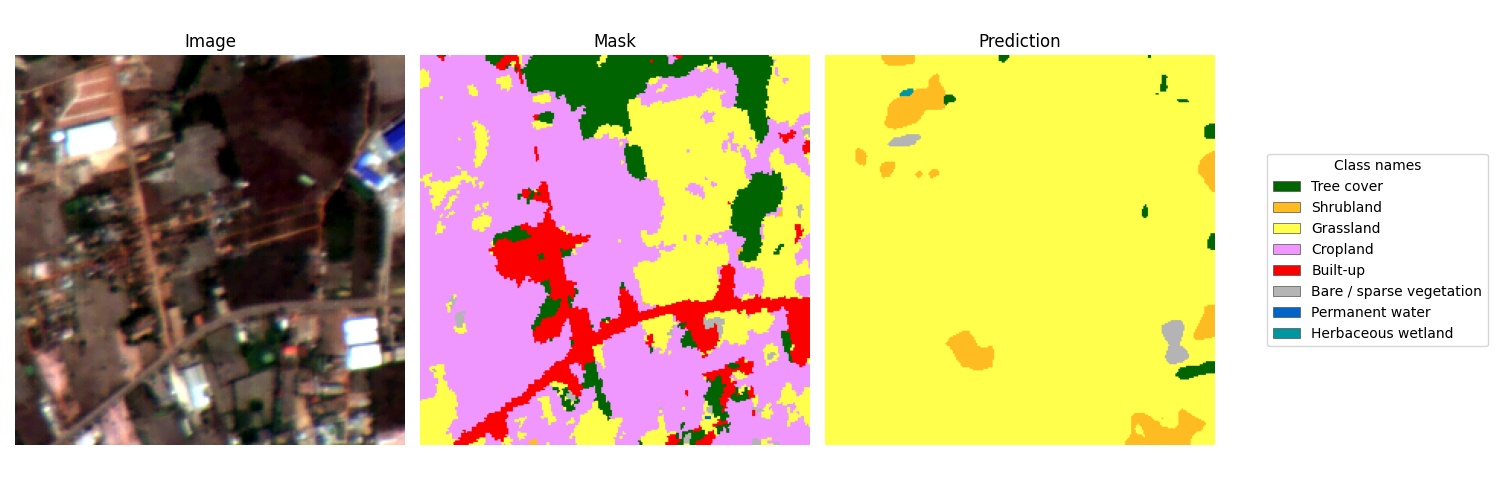
\includegraphics[width=\textwidth]{figures/media_images_samples_4_e83632d014201d2d1873.png}
    \caption[Qualitative Baseline Results]{Sample prediction from real $\Phi$-sat-2 test set of the TerraMind Base model fine-tuned on Sentinel-2.
        The model is unable to generalize to the new sensor and predicts grassland for the entire scene, which is the most common class in the training set. 
    }
    \label{fig:qualitative-baseline}
\end{figure}

\begin{figure}[htbp]
    \centering
    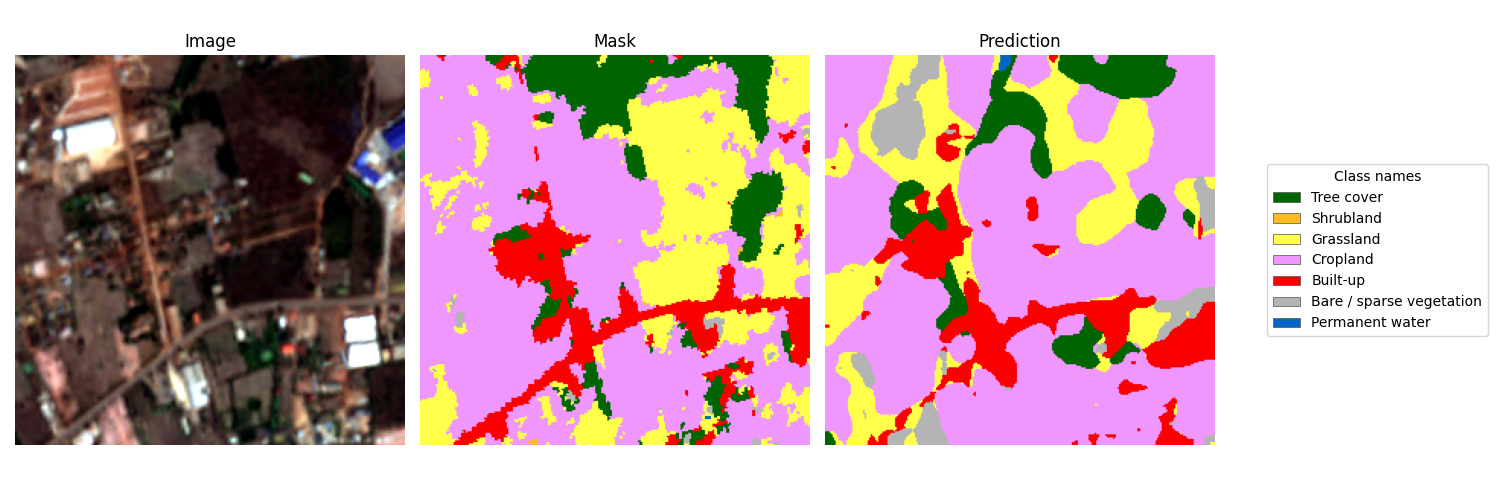
\includegraphics[width=\textwidth]{figures/media_images_samples_4_063cefee1b03274392e7.png}
    \caption[Qualitative Sentinel-2 Results]{Sample prediction from the Sentinel-2 patch of the same scene as of Figure~\ref{fig:qualitative-baseline}, from the TerraMind Base model fine-tuned on Sentinel-2.
        The model is able to correctly predict the classes of the scene, which shows that the poor performance on $\Phi$-sat-2 is not due to a difficult scene or a poor model, but rather to the domain gap between the two sensors.
    }
    \label{fig:qualitative-baseline-s2}
\end{figure}